\documentclass{article}
\usepackage[utf8]{inputenc}

\title{GitHub: a Short Practical Introduction}
\author{Last edited by: Luigi Caloi}
\date{December 2018}

%\graphicspath{ {./Figures/} }
\usepackage [english]{babel}
\usepackage [autostyle, english = american]{csquotes}
\MakeOuterQuote{"}
\usepackage{graphicx} 
\usepackage{csvsimple}
\usepackage{enumitem}
\usepackage{natbib}
\usepackage{graphicx}
\usepackage{array}
\usepackage{tabu}
\usepackage{longtable}
\usepackage{hyperref}
\usepackage{float}
\usepackage{booktabs,caption}
\usepackage[flushleft]{threeparttable}
\usepackage[utf8]{inputenc}
\usepackage{keystroke}
\usepackage{background}
\usepackage{etoolbox}
\usepackage{booktabs}
\usepackage{tabularx}
\usepackage{subcaption}
\usepackage[margin=1in]{geometry}
\hypersetup{
    colorlinks=true,
    linkcolor=blue,
    filecolor=magenta,      
    urlcolor=blue,
}

\makeatletter
\patchcmd{\tableofcontents}{\@starttoc{toc}}{\hypertarget{totoc}{}\@starttoc{toc}}{}{}
\makeatother

\backgroundsetup{
scale=1,
angle=0,
color=black,
position=current page.south,
vshift=20pt,
contents={
  \tikz[remember picture,overlay]
    \node[inner sep=0pt] {\hyperlink{totoc}{\Return}};
  }
}

\begin{document}
\maketitle
\tableofcontents

\begin{abstract} 
	This is a very short and practical introduction to GitHub intended to future RAs and co-authors. Most of commands for GitHub are very well documented online and you should have no problems to find them, but what can be sometimes tricky is understanding how to start using GitHub. I will briefly describe the main concepts of GitHub and try to illustrate the most important tools using one practical example. After reading this introduction you should be able to use GitHub in a project straight away. The idea is to give you an understanding of the main tools, so that you can later get a deeper understanding of them through online documentation. I recommend several website for specific tools along the way, but the most complete reading is \href{https://git-scm.com/book/en/v2}{Pro Git - Everything You Need to Know About Git} %\cite{1}. 
\end{abstract}

\section{Introduction - Please Read It}
	 
    In ``GitHub: a Practical Introduction'' I attempted to follow each explanation of Github's workflow and commands with an example on how to use them. If you want to follow the example and practice the commands, please email me at luigicaloi@gmail.com so I can grant you a ``collaborator access'' to the GitHub repository for this introduction. You will need it in order to perform some of the commands. \\
    \newline
    In the following sections I will guide you through (i) editing an existing project in Git and (ii) creating a project of your own and transferring it to Git. Although the examples are very simple, the commands are the same that you'll be using in more complex projects.
    
\section{GitHub Basics}

\subsection{Distributed Version Control System}
	As you probably know, GitHub is a Version Control System (VCS) -- it stores in repositories (often called repos) all the versions from your project that you saved, so you don't lose your project's history. However, a key feature of GitHub that differentiates it from older VCSs is that it is a Distributed VCS. This means that GitHub not only stores a version of your project on its cloud service (called remote repo), but also every user from a project stores the entire history of the project on their computers. So besides storing the current version of the project that you are working on (called the working directory), you also store a Git repository on your computer with the project's history (called the local repo). \\
    \newline
	This allows GitHub to work (i) incredibly fast, since it doesn't have to access the internet to access a project's history; (ii) independent from your internet connection, for the same reason, and (iii) very safely, since every user serves essentially as a backup of the project's history. This also explain why most users keep their code in a GitHub folder and their data on a storage system (e.g. DropBox)--it would be too costly to save multiple versions of your datasets to your computer. \\
    
    \begin{figure}[H]
    	\caption{Distributed Version Control System}
    	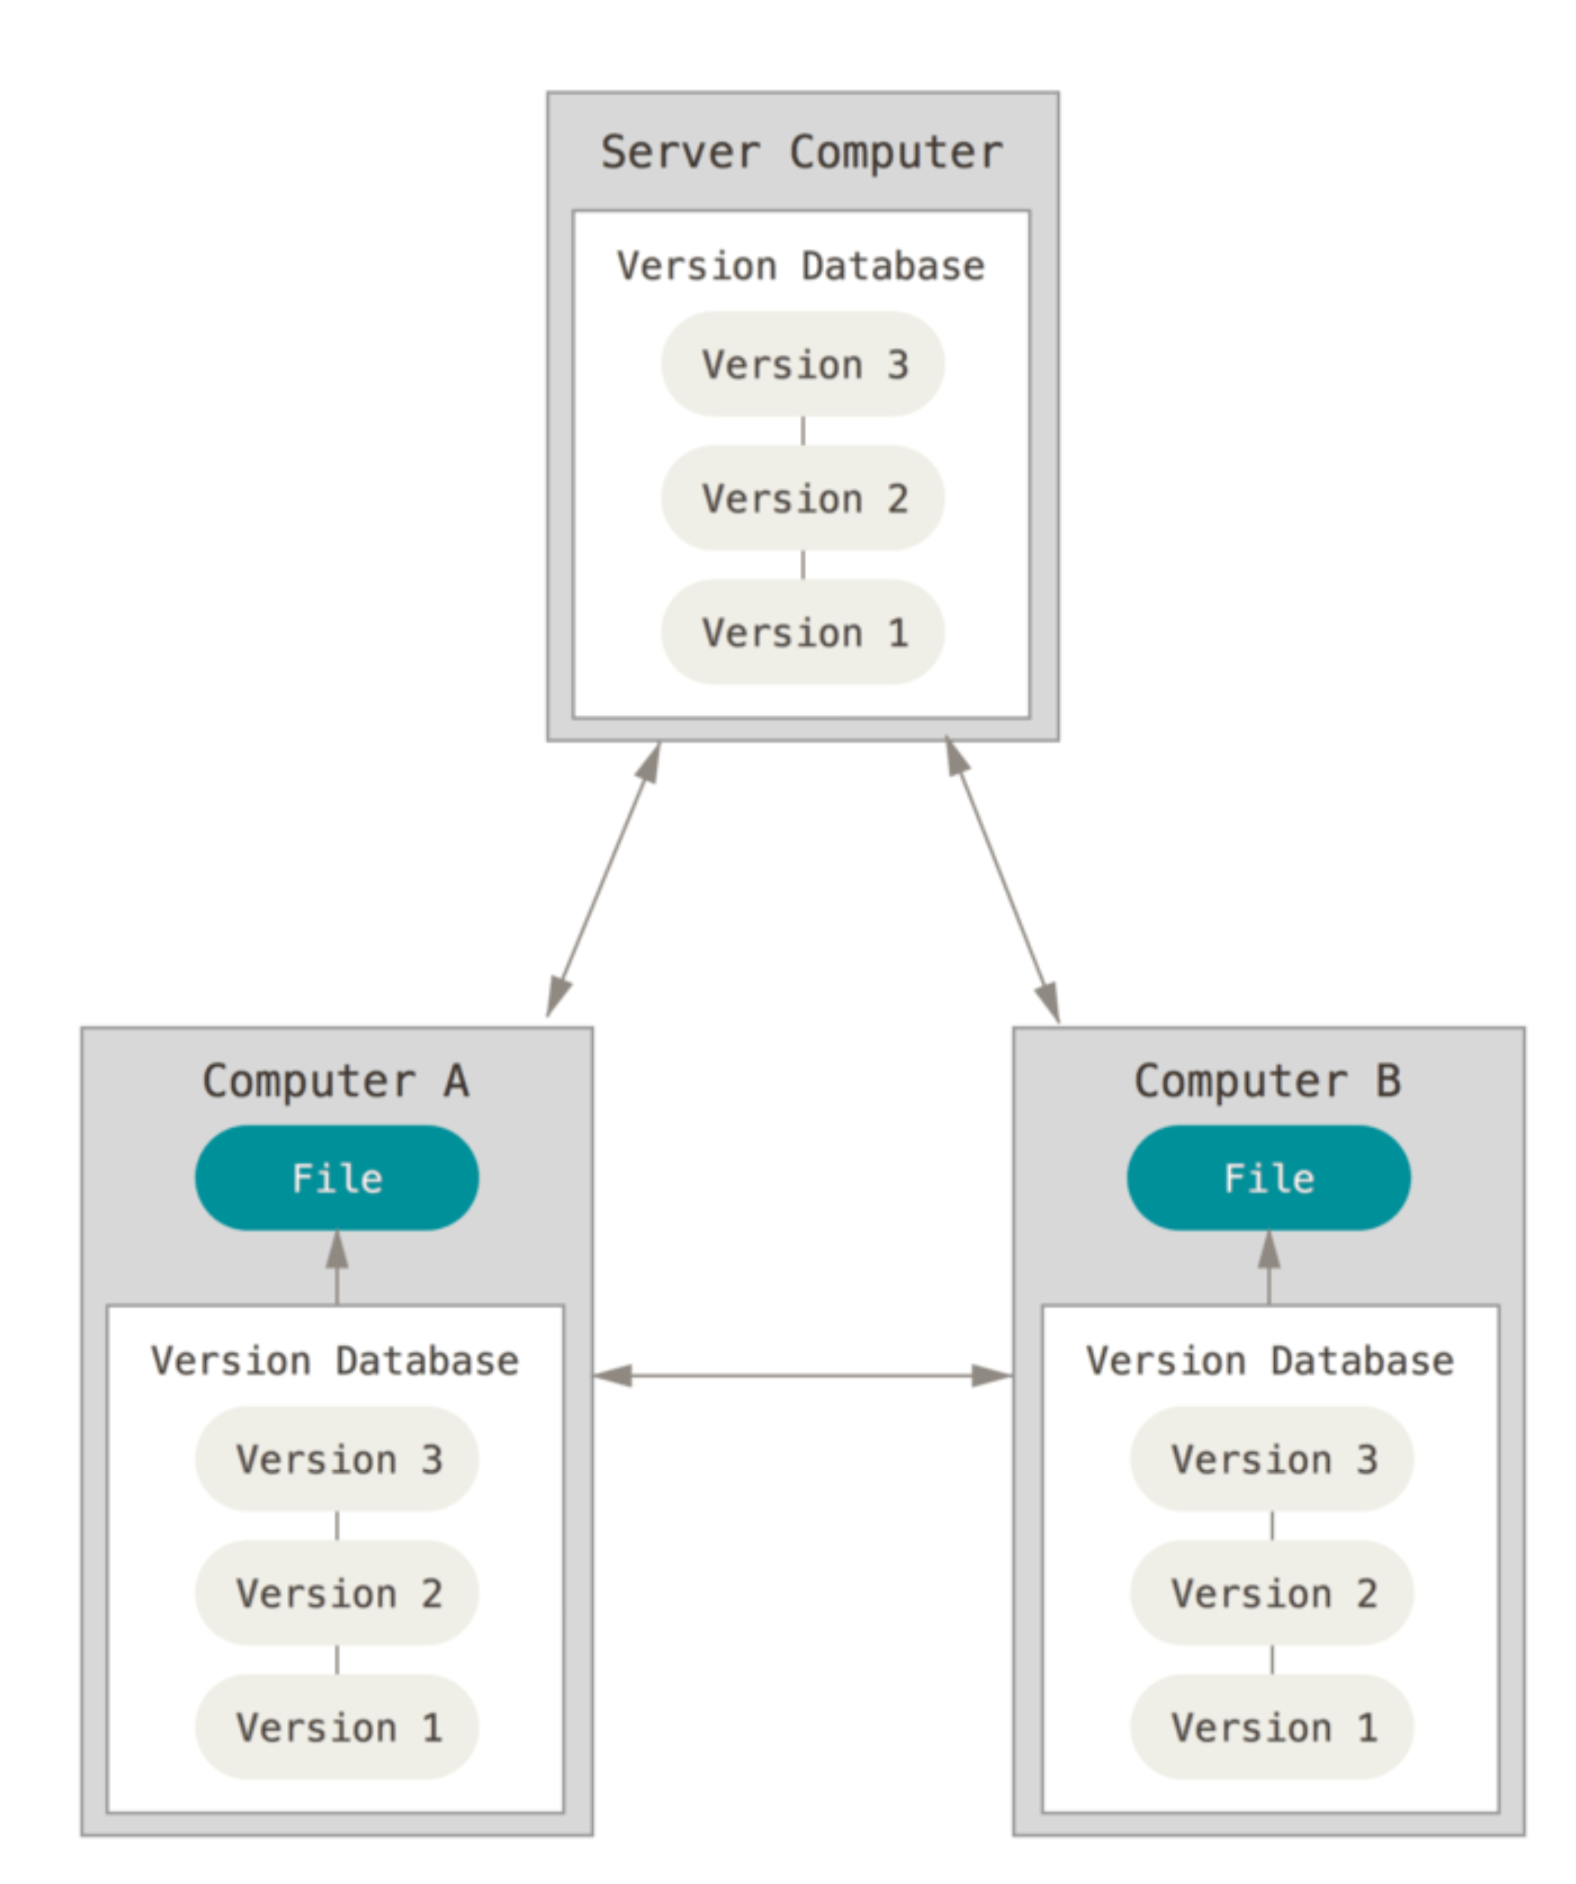
\includegraphics[scale=0.3]{images/figure1.png}
	    \centering
    \end{figure}
    
	In figure 1 above, the Version Database is what we call the ``remote repo.'' The Files in Computer A and in the Computer B are the ``working directories'' and the Version Database in each computer are the ``local repos.'' Local repos, or .git repos, are by default hidden in your computer, so you'll only see your working directory. From this point onward we will see how to create local and remote repos to store your project's history.


\subsection{Git Setup}
    \begin{itemize}
        \item First step: install the program. You can find very simple instructions \href{https://git-scm.com/book/en/v2/Getting-Started-Installing-Git}{here}. 
        \item Second step: create an account on \href{https://github.com}{GitHub}
        \item Third step (optional): setup your identity. Go to your terminal and type the following commands: \\
        \newline
        \indent \$git config --global user.name ``John Doe'' \\
        \newline
        \indent \$git config --global user.email johndoe@example.com \\
        \newline
        Don't actually copy the \$ symbol, this is standard notation to let you know this command should be run in the terminal. If you need any help to understand a command, you can type the git help $<$verb$>$. For instance: \\
        \newline
        \indent \$git help config
    \end{itemize}

\section{Joining a Project: Cloning an Existing Repo}

    This section guides you through an example on how to join an existing project, probably that your co-author or Professor already began. This will be useful to introduce some concepts and Git commands. It will also be all that RAs will need to know 90\% of the times.
    
\subsection{Clone a repo}

    To clone a repository means that you are reaching out to a remote repository and copying nearly all data that the server has into a new local repo in your computer. Let's illustrate this with an example:
    \begin{itemize}
        \item First step: access the url of the \href{https://github.com/luigicaloi/GitShortIntro}{remote repo}.
        \item Second step: Open terminal
        \item Third step: Go to the directory where you want your repo to be: \\
        \newline
        \indent \$ ``cd /Users/username/documents''
        
        \item Fourth step: Go to the \href{https://github.com/luigicaloi/GitShortIntro}{remote repo}, click on clone or download and copy that link displayed. \\ 
        \newline 
        Then, on your terminal, clone the repository with git clone $<$ulr$>$   \\
        
        \indent \$ git clone  ``https://github.com/luigicaloi/GitShortIntro.git'' \\
    \end{itemize}
    This will create a GitShortIntro directory with a working copy of the latest version of the project. It also stores a .git directory (the local repo) inside it, which is hidden. For more info, see \href{https://help.github.com/articles/cloning-a-repository/}{this}.
    
    \subsection{Modifying Files}
    If you open the new GitShortIntro directory, you'll see that there are only two files, ``AllReaders.tex'' and ``Test.do,'' and one folder ``GitHub\_a\_Practical\_Introduction''. Your task is simple: open the ``AllReaders.tex'' file and include your name at the end of the list of all readers. \\
    \newline
    Now that you have made changes to the working directory, let's see what is your status in Git. Change the directory in the terminal for the one from your new project. For instance: \\
    \newline
    \indent \$ cd ``/Users/username/documents/GitShortIntro'' \\
    \newline
    and write the following command on the terminal: \\
    \newline
    \indent \$ git status \\
    \begin{figure}[H]
	\caption{Git status}
	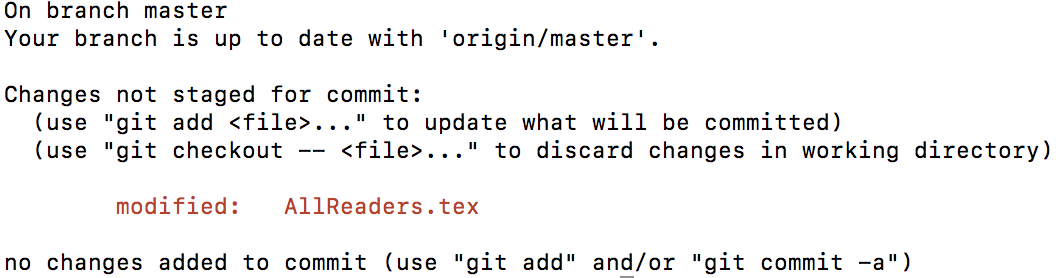
\includegraphics[scale=0.5]{images/figure2.png}
	\centering
    \end{figure}
    Don't worry about the branch message yet, we'll see what that is in section \hyperref[sec:branching]{Git Branching}. GitHub realizes that your local repo is different from your working directory, it realized that you made changes to the ``AllReaders.tex'' file and shows it under ``Changes to be committed.'' Our first goal is to make sure that your local repo also saves those changes (we'll take care of the remote repo in the next section). You first need to tell GitHub what documents you want to save the changes in the local repo with the following command: \\
    \newline
    \indent \$ git add ``AllReaders.tex''
    \newline
    \newline
    Now run git status again and you'll see:
    \newline
    \begin{figure}[h]
	\caption{Git status}
	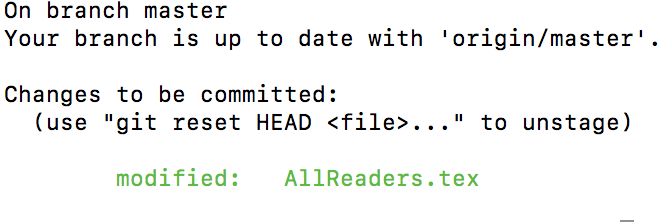
\includegraphics[scale=0.5]{images/figure3.png}
	\centering
    \end{figure}
    \subsection{Committing Modified Files}
    AllReaders.tex is now under the ``Changes to be committed.'' This basically means you told GitHub you want to save the changes made to it. Next, we need to ``commit'' those changes. Committing is telling GitHub to take a snapshot of your project in the working directory and save it to your local repository. In other words, you are saving your latest changes to the git repo.
    See \href{https://git-scm.com/docs/git-commit}{here} here for more details. The command to commit changes is: \\
    \newline
    \indent \$ git commit -m ``A message explaining your changes to the project''
    \subsection{Unmodifying a Modified File}
    If you accidentally modified a file, or regretted the changes, and wants to revert it back to how it was when you last committed (the local repo's last snapshot), you can run the following command: \\
    \newline
    \indent \$git checkout -- $<$file$>$ \\
    \newline
    However, be careful, the changes you had made and not committed will be completely deleted.
    \subsection{Pushing to Your Remotes}
    \label{sec:pushing}
    So you have already (i) cloned all the data from the remote repo and created a local repo; (ii) modified your working directory and (iii) added and committed your changes from your working directory to your local repo (the .git repository). We'll now update your changes to the remote repo. This can be done with the following command: \\
    \newline
    \indent \$git push origin master \\
    \newline
    Or more generally \\
    \newline
    \indent \$git push $<$remote$>$ $<$branch$>$ \\
    \newline
    ``origin'' is the automatic name that GitHub assigns to the remote repository. ``master'' is the branch in the remote repo, but don't worry about it yet, it will make sense after we see \hyperref[sec:branching]{Git Branching}. Git push uploads the changes from your local repo to your remote repo. Now your working directory, your local repo and your remote repo are all on the same stage.
    \section{Creating a Repo}
    \subsection{Creating an Empty Repo}
    In the last section we saw how to clone a repo, make changes to your local repo and push it back to the remote. In this section we will simply see how to create an empty remote repo, then you can follow the workflow from Section 3 to add your files to it.
    \begin{itemize}
        \item First step: Go to GitHub's website and login.
        \item Second step: On any page, click the + button on the upper right part of the screen and then click on ``New repository.''
        \item Third step: Choose the name of your repo and click Create repository.
    \end{itemize}
    For more options, see \href{https://help.github.com/articles/creating-a-new-repository/}{this}.
    \subsection{Adding an Existing Project to Your New Repo}
    To add an existing project to the new remote repo, we will first create a local repo, add the existing project to it, commit the changes and push it to the empty remote repo. 
    \begin{itemize}
        \item First step: Change the current working directory to the desired local's project dir. \\
        \newline
        \indent \$cd /Users/username/newrepo
        \item Second step: Initialize a local git repository in your current directory \\  
        \newline
        \indent \$git init
        \item Third step: Add the files for your new repo
        \item Fourth step: Commit the new files, which creates a snapshot of how they are now and save it to the local repo
        \item Fifth step: Go back to your remote repo on GitHub's website and copy the remote repository URL.
        \item Sixth step: Add the new remote repo from your terminal
        \indent \$git remote add origin $<$remote repository URL$>$
        \item Seventh step: Your local repo is now connected to your remote repo. Push your changes to your remote repo as we saw in \hyperref[sec:pushing]{Pushing to Your Remotes}.
    \end{itemize}
    For more details and options, see \href{https://help.github.com/articles/adding-an-existing-project-to-github-using-the-command-line/}{this}.
    \section{Branching and Merging}
    In this section we will see the two concepts that are most important for collaborative work -- branching and merging.
    \subsection{Git Branching}
    \label{sec:branching}
    The easiest way to understand branches is to think about the repo as a series of commits. When you create a repo, GitHub automatically creates a branch called master. This branch is simply a pointer to the last commit of your project. In figure 4 bellow, for instance, the master branch is pointing to the third and last commit (C2).
    \begin{figure}[H]
    	\caption{Branch Master}
    	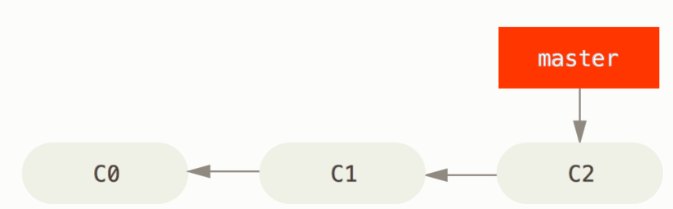
\includegraphics[scale=0.5]{images/figure4.png}
    	\centering
    \end{figure}
    \leavevmode \\
    Now let's say that you need to make changes to your project for a new submission, but you don't want to change the original code yet. You  can create a new branch, called testing, with the following command \\
    \newline
    \indent \$git branch testing \\
    \begin{figure}[H]
    	\caption{New Branch}
    	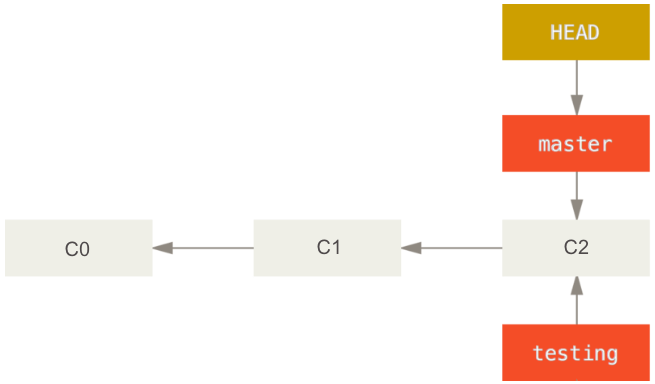
\includegraphics[scale=0.5]{images/figure5.png}
    	\centering
    \end{figure} 
    \vspace{0.2 in}
    Now the two branches are pointing to the last commit (see figure 5 above). The HEAD pointer shows which branch you are currently working in your local repo.
    The following command switches control to the testing branch so that you can make the new changes to your project. \\
    \newline
    \indent \$git checkout testing \\
    \newline
    Now if you make changes to your project and commit them, your project history will look like Figure 6. Note that the master branch is still pointing to commit C2.
    \vspace{0.2 in}
    \begin{figure}[h]
    	\caption{New Branch}
    	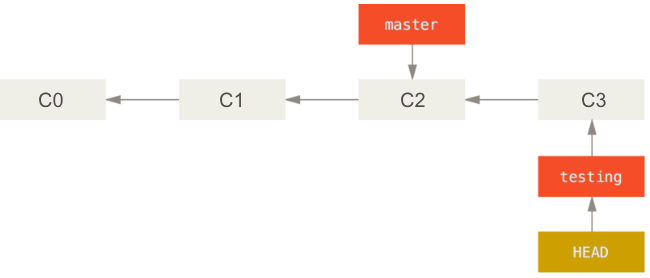
\includegraphics[scale=0.5]{images/figure6.png}
    	\centering
    \end{figure} 
    \vspace{0.2 in}
    The good thing is that if we decide that the new ideas were bad, we can simply go back to the master branch with \\
    \newline
    \indent \$git checkout master \\
    \newline
    With this, all the files on your working directory go back to how they were when you made the last push in your master branch (C2). \\
    \newline
    Another scenario that illustrates why it is good to make new changes in new branches is when a journal asks you to make a change some details to a paper in which you have been making drastic changes to. You can easily go back to your `master' version (assuming this is the one you submitted to the journal), make changes to it, and then go back to your 'testing' branch to continue working on the big changes.
    \subsection{Git Merging}
    Following from last subsection's example, let's suppose that while you made changes to the `testing' branch, someone else had to make urgent changes to the master branch. For that, this person created a `hotfix' branch. The history of your project now looks like this: 
    \begin{figure}[H]
	\caption{New Branch}
	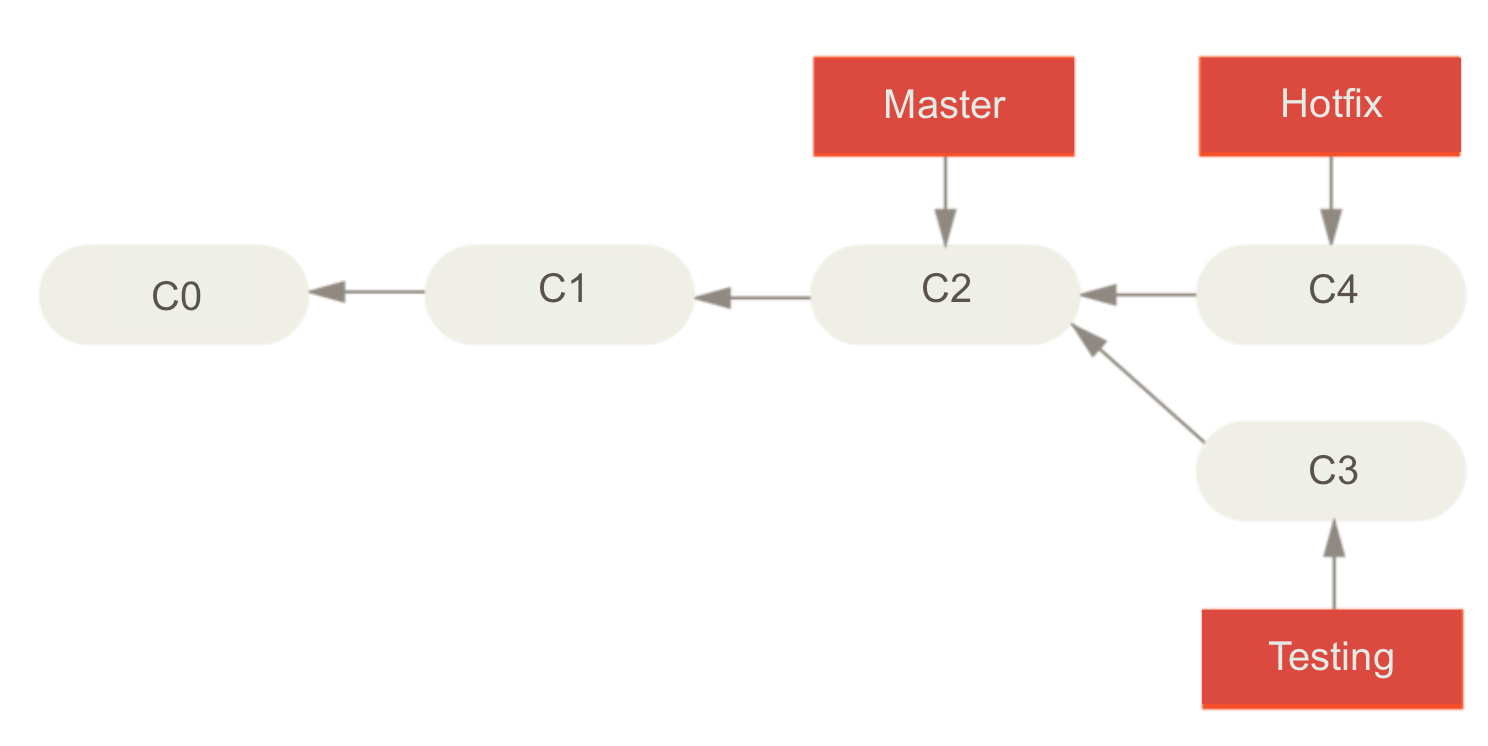
\includegraphics[scale=0.5]{images/figure7.png}
	\centering
    \end{figure} 
    Now let's say we finished the changes in the hotfix branch and we are ready to merge the master branch with the hotfix branch. This can be done with the following command:\\
    \newline
    \indent \$git checkout master \\ 
    \newline
    \indent \$git merge hotfix \\
    \newline
    And we would see the following message:
    \begin{figure}[H]
    	\caption{New Branch}
    	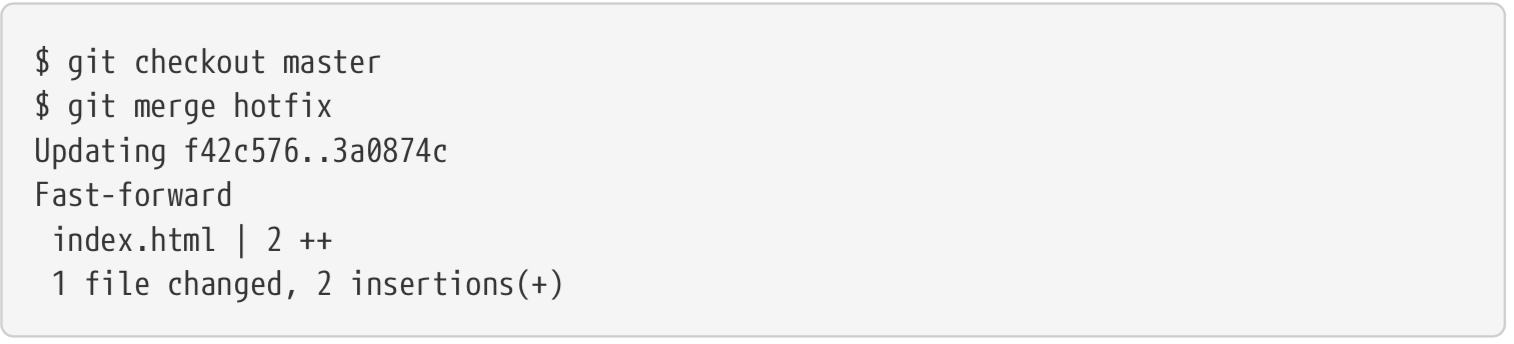
\includegraphics[scale=0.5]{images/figure8.png}
    	\centering
    \end{figure} 
    \vspace{0.2 in}
    Because we didn't make any changes to the master branch and C4 from the hotfix branch was directly ahead of C2, GitHub can simply "fast-forward" the master branch and change the pointer from C2 to C4. Since the hotfix branch and the master branch now point to the same commit, we can delete the hotfix branch: \\
    \newline
    \indent \$git branch -d hotfix 
    \subsubsection{Merging conflicts}
    Things are a bit more complicated when you are trying to merge two branches that are not directly related. For instance, if some changes made in the hotfix branch are in conflict with changes made in the testing branch, GitHub won't be able to complete the merge and will ask your help to decide which version it should keep for that specific change. \\
    \newline
    The first step would be to try merging both branches. \\
    \newline    
    \indent \$git merge testing \\
    \newline
    We would then check in which files there was a merge conflict with git status   
    \begin{figure}[H]
    	\caption{New Branch}
    	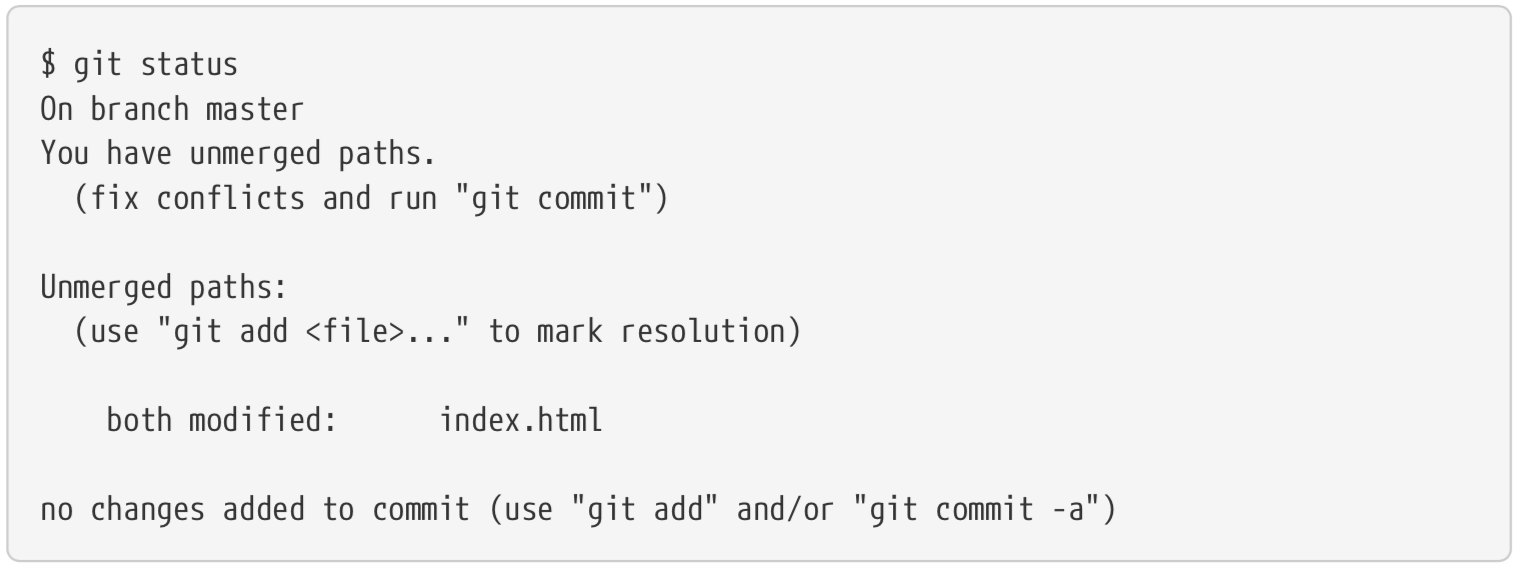
\includegraphics[scale=0.5]{images/figure9.png}
    	\centering
    \end{figure} 
    Any file with a merge conflict would be under `unmerged paths'. To solve the conflicts, we first need to open the files in a text editor. GitHub adds conflict resolution markers in it so that we can solve the conflict manually. For instance, in the `index.html' file from the example above, the section of the file that must be solved looks like this:
    \begin{figure}[H]
    	\caption{New Branch}
    	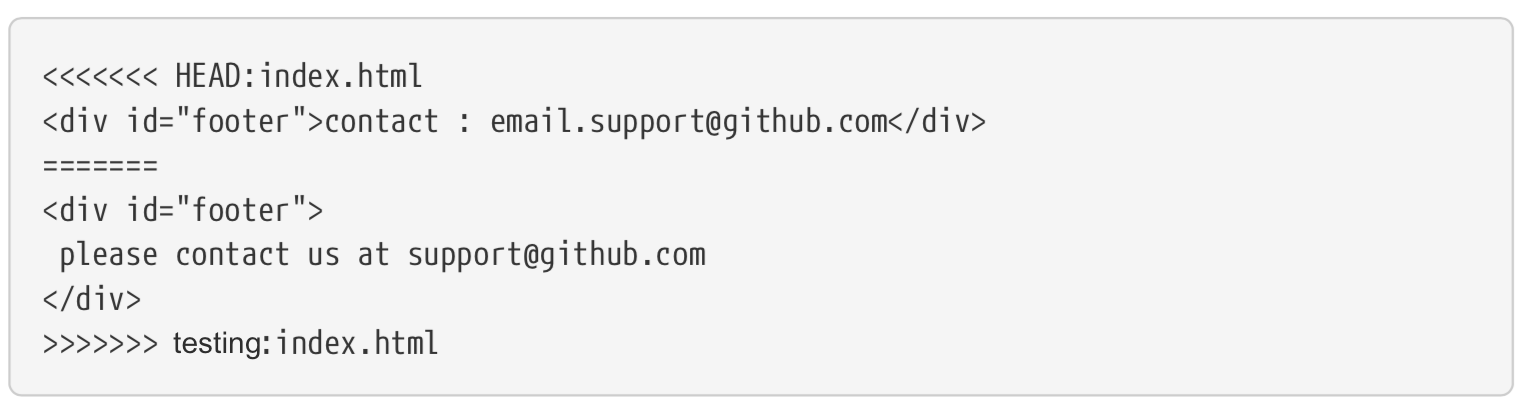
\includegraphics[scale=0.5]{images/figure10.png}
    	\centering
    \end{figure} 
    The changes made to the master branch are under $<<<<<<<<$ HEAD:index.html and above the ======= lines, because HEAD was pointing to the master branch (i.e. the user was in the master branch). Everything bellow $<$div id=``footer''$>$ and above  $>>>>>>>$ testing:index.html was in the testing branch. You can manually solve this issue by keeping the version you prefer, or a combination of both. Of course, delete the conflict signals from GitHub. \\
    \indent For instance, one way to solve this issue would be to substitute the entire block with this:
    \begin{figure}[H]
    	\caption{New Branch}
    	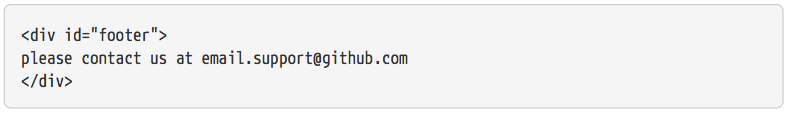
\includegraphics[scale=0.5]{images/figure11.png}
    	\centering
    \end{figure} 
    Once you're done solving the conflicts, the next step would be to let Git know these files are solved by running git add in the terminal. \\
    \newline
    \indent \$git add document
    \newline
    \newline
    You can then commit your changes and finish merging the two branches.
    For more details, please see \href{https://git-scm.com/book/en/v2/Git-Branching-Basic-Branching-and-Merging}{this}.
    When merging branches that are not directly linked, instead of just moving the branch pointer forward, GitHub will create a new commit that includes the changes in hotfix and testing. Your new commit history will look like this:
    \begin{figure}[H]
    	\caption{New Branch}
    	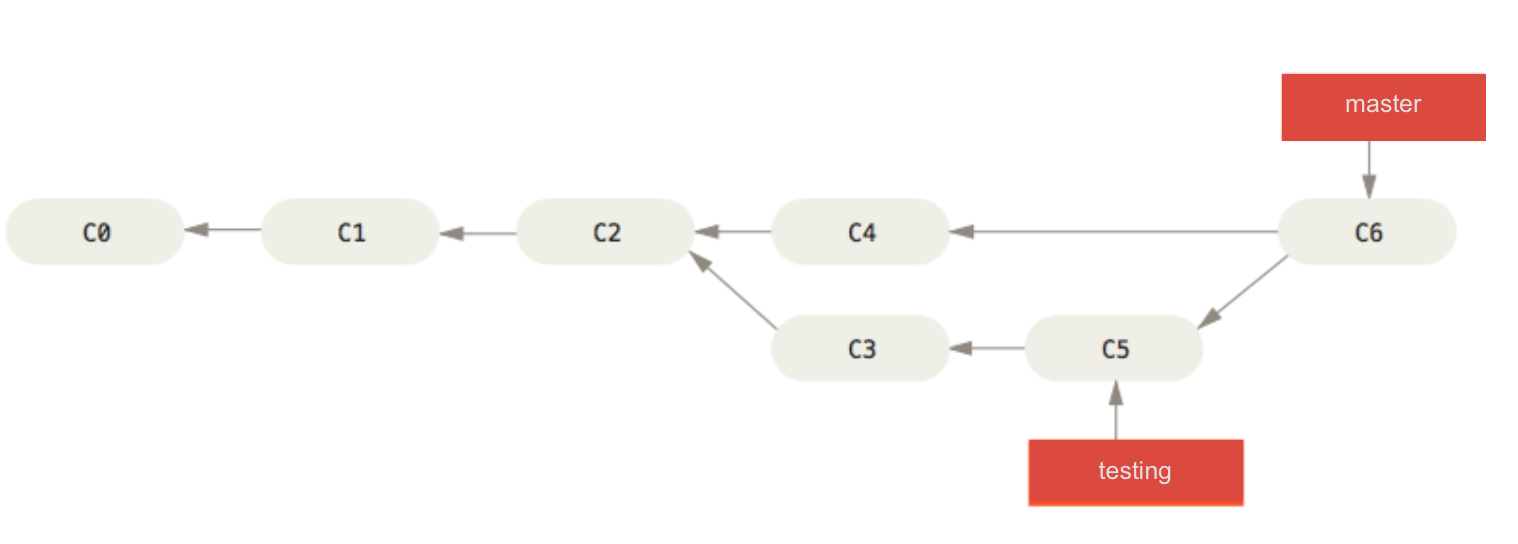
\includegraphics[scale=0.5]{images/figure12.png}
    	\centering
    \end{figure} 
    Branching and merging allow us to understand better what was going on with the push command in \hyperref[sec:pushing]{Pushing to Your Remotes}. We saw how to push a local repository to a remote one with the command git push $<$remote$>$ $<$branch$>$, but I asked you not to pay attention to what was the branch part of it. Just like our local repo, the remote repo can have multiple branches (they usually follow the same structure as our local repo). The $<$branch$>$ command is simply telling Git to what branch of our remote repo we want to push our changes. Second, it might have seemed like Git magically sent the data to the remote repo and made both be on the same stage. What if there are three people working on the same branch and pushing their changes to the branch in the remote repository? The push command is implicitly merging the local and remote branches. Therefore, if there are multiple people pushing to the same branch, we might need to fix merge conflicts to decide what changes to keep.
    \section{Using GitDesktop}
    \label{sec:GitDesktop}
    While using the terminal can be very good to work on GitHub, the GitDesktop app is useful for visualizing what changed in a new push. 
    \begin{itemize}
        \item First, download GitDesktop  \href{https://desktop.github.com/}{here}.
        \item Second, add your local repository to the GitHub Desktop by going to File $\rightarrow$ Add Local Repository.
        \item Third, on the left of your screen, choose GitShortIntro as your current repository and master as your current branch.
        \item Fourth, click on pull origin to make sure that your GitHub Desktop is up to date with the remote repo.
        \item Fifth, Under your current repository, click on "history."
    \end{itemize}
    This is a list of the commits to that repository to the master branch on the GitShortIntro remote repository. You can click in one of the commits to see what changes were made. In red are the deleted lines and in green that ones that were added. 
    \begin{figure}[H]
    	\caption{GitHub Desktop}
    	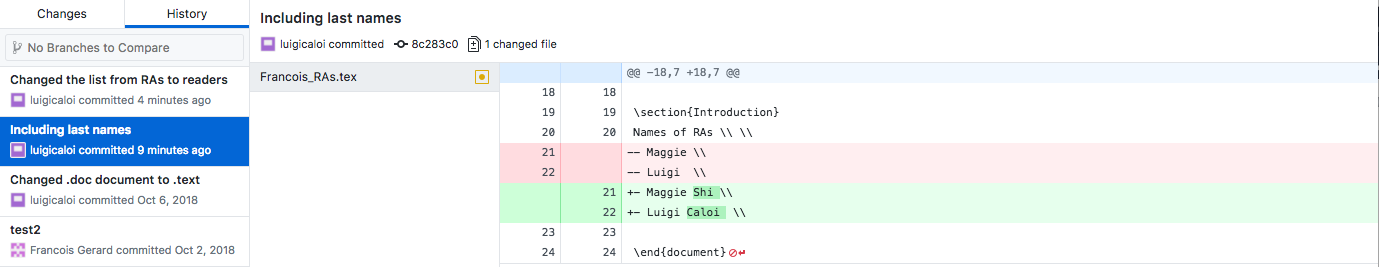
\includegraphics[scale=0.5]{images/figure13.png}
    	\centering
    \end{figure} 
    
\section{Workflow}
There are several types of workflow in Git, many of which we indirectly covered in the previous sections. Here I'll focus on the (i) centralized workflow and (ii) xxx workflow, but for more details please see \href{https://www.atlassian.com/git/tutorials/comparing-workflows}{this}.

\subsection{Centralized Workflow}
The centralized workflow is the simplest and the easiest to transition for who's been using DropBox. The idea is quite simple: the entire project has only one branch, the master branch, which all changes are committed into. This branch serves as central repository and you "push" your changes similarly to when you want sync your code to the DropBox folder. 

\begin{figure}[H]
	\caption{Master branch and multiple users}
	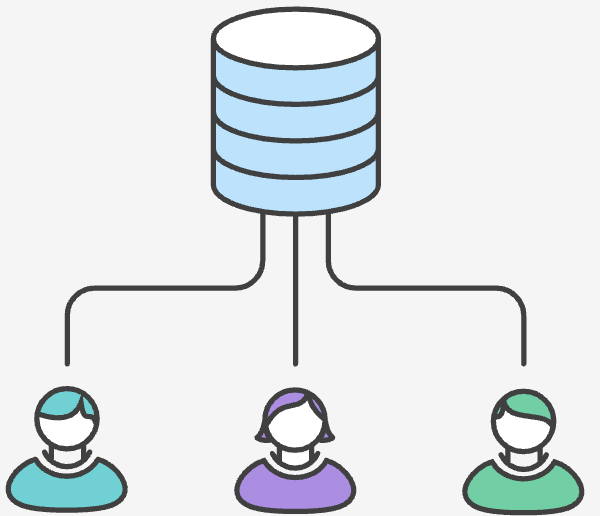
\includegraphics[scale=0.5]{images/CentralizedWorkflow.png}
	\centering
\end{figure}

Despite its simplicity, the centralized workflow with Git already offers some advantages compared to other repository systems:

\begin{enumerate}
    \item It allows each developer/researcher to work independently of all other changes to a project. E.g. you can work in the same .do file (or other code) as another colleague without worrying if DropBox will mess up the changes made by both of you.
    \item Merging two researcher's work is much easier: Git provides a useful merge conflict functionality that allows one to see what parts of the code of each researcher need to be fixed in a merge. 
    \item It allows one to control when he/she wants to share the changes in his/her code. I.e. while a code that is stored in DropBox is constantly being synced  and updated to everyone, in Git you gain more control by making edits to the code in your computer (local repo) and deciding when to push the changes to the remote repo.
    \item It gives every developer their own local copy of the entire project
\end{enumerate}

Please see \href{https://www.atlassian.com/git/tutorials/comparing-workflows#centralized-workflow}{this} for more details.

\subsection{Feature Branch Workflow}

In short, the Feature Branch Workflow requires an ``official'' branch (usually the master branch) to store all stable and accepted code, while the development of new features to the code should take place in dedicated separate branches. \\
\newline
In \hyperref[sec:branching]{Git Branching} we already illustrated the feature branch workflow. If you recall, we mentioned that you could (i) create a `testing' branch to create new features to your code while keeping your main code intact or (ii) create a `hotfix' branch. The examples in that section illustrate the benefits of the Feature Branch Workflow:

\begin{enumerate}
    \item \textbf{Collaboration:} It makes it easy for multiple researchers to work on a particular feature while keeping the main codebase intact. While the Centralized Workflow allows more control compared to DropBox--a researcher can choose when to ``push'' changes to the master branch--the ``feature branches'' allow multiple users to collaborate before making the changes official in the master branch.
    \item \textbf{Stability:} By definition it guarantees that the master branch always have official and bug-free code. After all, you should merge your ``feature'' branch to the master branch once the feature became official and stable.
    \item \textbf{Organization of progress:} Since all new code features are developed in separate branches and only the accepted stable codes are merged to the master branch,  the master branch provide an offician history of the project development.
\end{enumerate} 
\textbf{Alternative:} If creating a new branch whenever you will create a new feature seems a bit cumbersome, a simpler alternative is to create branches for each one of the project collaborators. In this strategy, the branch ``John'' will reflect the work John is doing. If Sophia wants to help him she can easily access John's code state by switching to John's branch.

    
\section{Some Final Tips}
The biggest advantage of GitHub is to help a group of multiple people to coordinate their work in one single code. A few notes are worth making:
\begin{itemize}
    \item It is a good practice to push/pull your changes to the remote repo at least weekly to make sure you have the latest updates of your branch.
    \item Try to divide your `commits' into small changes to make them cohesive. E.g. in \hyperref[sec:GitDesktop]{Using GitDesktop}'s picture it was easy to understand what changed in the latest commit--Last names were added to the list of names--but it would be hard to understand what happened if multiple changes to multiple codes had been made.
    \item Keep your GitHub folder outside of DropBox--it can get confusing if your code is getting updated by DropBox or by the pull/push from GitHub.
    \item If you use the Feature Branch Workflow, aim for short-lived branches. The longer a branch lives, the higher the chances of confusing merge conflicts when merging it to the master branch.
\end{itemize}

\end{document}
    
    
    